% This file is intentionally modular: it can be included from the standalone
% SVM report or copied into the team's final two-page report.

\section{Linear Support Vector Machine}

\subsection{Motivation and formulation}

The target is strongly imbalanced: only 28,975 of 328,135 training examples
(8.8\%) have the positive \texttt{\_MICHD} label. Consequently, the
all-negative classifier obtains 91.17\% validation accuracy while detecting no
positive cases. We therefore optimized a linear soft-margin support vector
machine (SVM) for balanced accuracy and positive-class recall rather than raw
accuracy alone. Given labels $y_i\in\{-1,+1\}$ and transformed features
$x_i$, the fitted model minimizes
\begin{equation}
  \frac{1}{N}\sum_{i=1}^{N}\alpha_i
  \max\!\left(0,1-y_i w^\top x_i\right)
  +\frac{\lambda}{2}\lVert w\rVert_2^2,
  \label{eq:weighted-svm}
\end{equation}
where $\alpha_i=N_-/N_+$ for positive examples and $1$ otherwise. This class
weight makes errors on the minority class more costly. We trained the primal
objective with stochastic subgradient descent, using only NumPy.

\subsection{Preprocessing and experimental protocol}

BRFSS survey responses contain categorical codes and feature-specific sentinel
values such as ``Don't know'' and ``Refused''. Treating these codes as ordinary
numbers would introduce false ordinal relationships. Our codebook-aware
pipeline converts verified sentinels to missing values, median-imputes and
standardizes numeric variables, adds numeric missingness indicators, and
one-hot encodes categorical variables with a separate missing category. All
statistics and categories are learned from the training partition only.

We used an 80/20 stratified holdout with seed 42, giving 262,508 training and
65,627 validation examples. The transformed validation experiment contained
1,194 columns including the intercept. Hyperparameters were selected through
a staged search over $\lambda$, positive-class weight, learning rate, and
number of updates. The final configuration was $\lambda=0.01$, learning rate
$10^{-4}$, 200,000 updates, and positive-class weight 10.3248.

\begin{figure}[t]
  \centering
  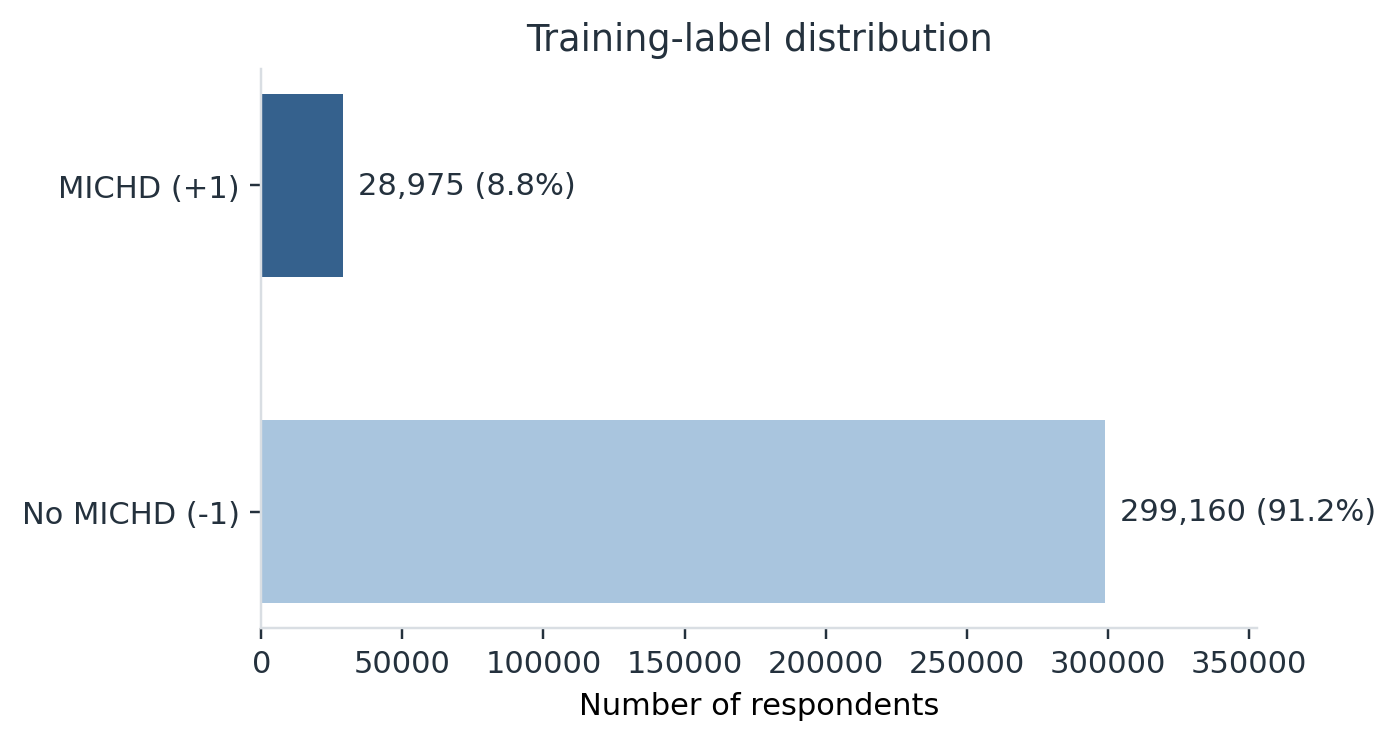
\includegraphics[width=0.82\linewidth]{assets/class_distribution.png}
  \caption{The strong training-label imbalance motivates class-sensitive
  evaluation and weighting. Counts are computed directly from the released
  training labels.}
  \label{fig:svm-class-distribution}
\end{figure}

\subsection{Results}

\begin{table}[t]
  \centering
  \caption{Complete-data holdout results. The dummy model illustrates why
  accuracy alone is misleading for this task.}
  \label{tab:svm-validation-results}
  \begin{tabular}{lrrrrrr}
    \toprule
    Model & Acc. & Bal. acc. & Prec. & Recall & F1 & Spec. \\
    \midrule
    All-negative & .9117 & .5000 & .0000 & .0000 & .0000 & 1.0000 \\
    Weighted SVM & .8062 & .7710 & .2747 & .7284 & .3989 & .8137 \\
    \bottomrule
  \end{tabular}
\end{table}

The weighted SVM correctly identified 4,221 of 5,795 positive validation
examples, corresponding to 72.84\% recall. It reduced ordinary accuracy because
11,147 negative examples were classified as positive, but improved balanced
accuracy from 0.5000 to 0.7710 and F1 from 0 to 0.3989. This is the intended
trade-off: the model detects substantially more at-risk respondents instead of
exploiting the majority class.

\begin{figure}[t]
  \centering
  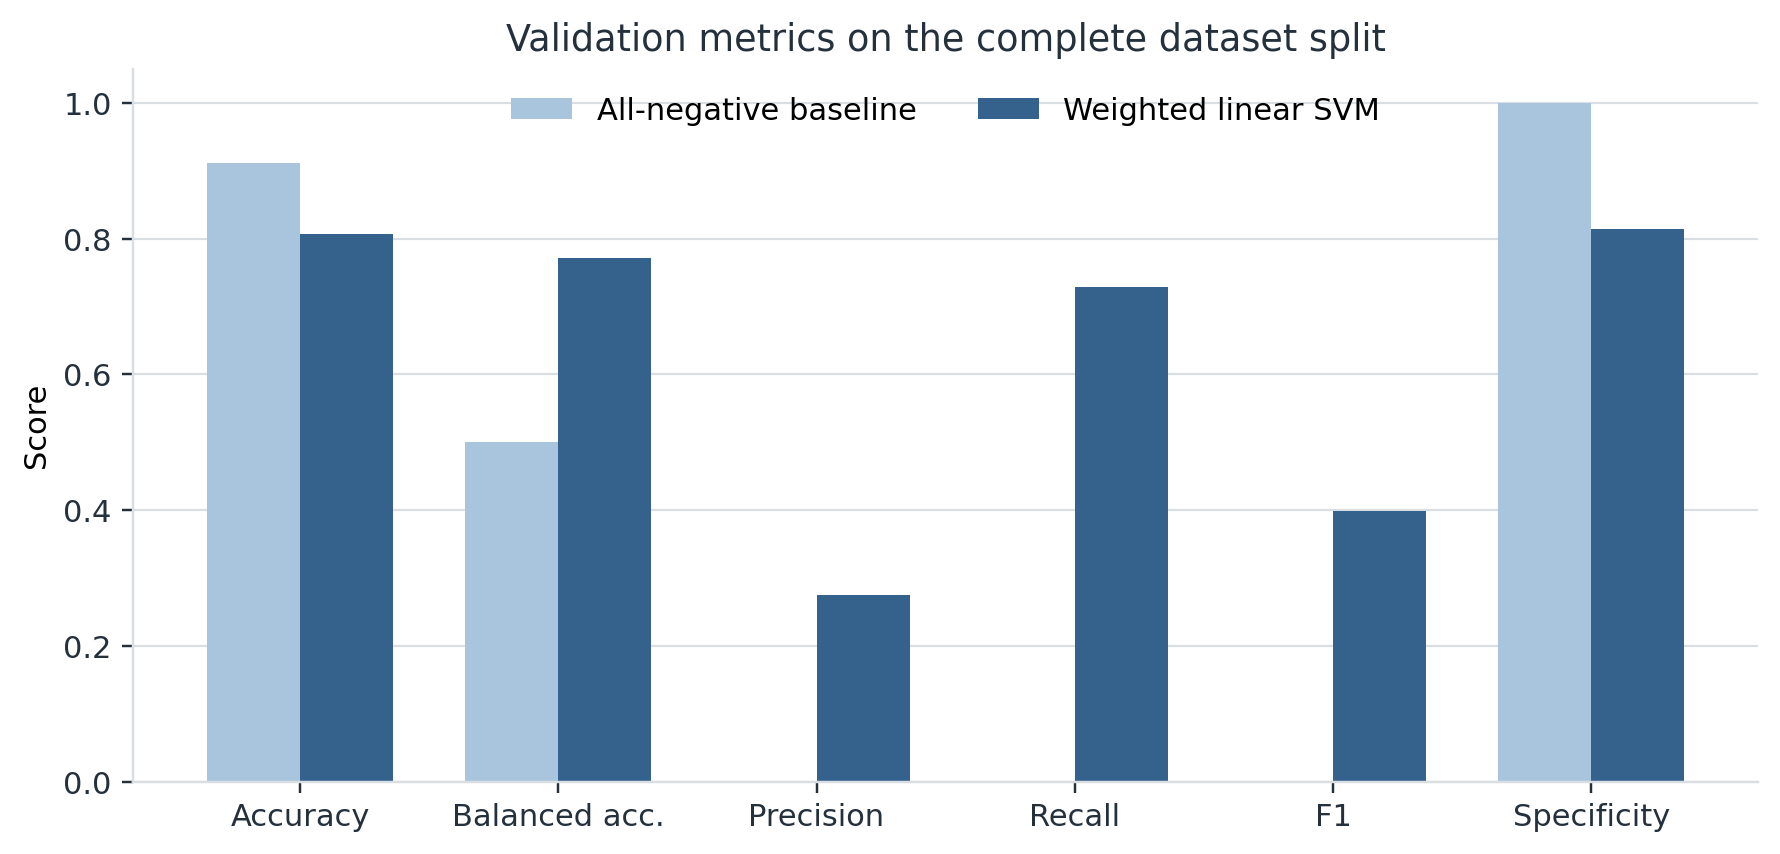
\includegraphics[width=0.92\linewidth]{assets/validation_metrics.png}
  \caption{Validation comparison between the all-negative baseline and the
  selected class-weighted linear SVM.}
  \label{fig:svm-metrics}
\end{figure}

\begin{figure}[t]
  \centering
  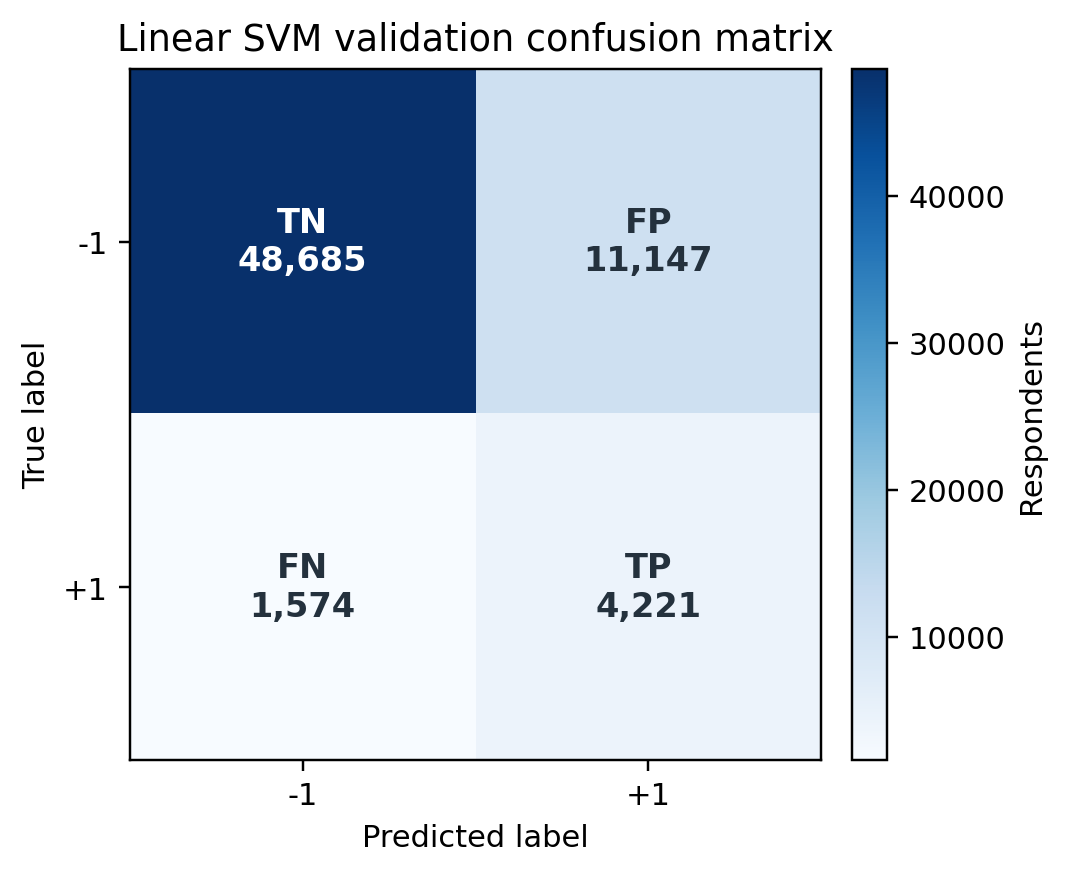
\includegraphics[width=0.62\linewidth]{assets/confusion_matrix.png}
  \caption{Validation confusion matrix for the selected SVM configuration.}
  \label{fig:svm-confusion}
\end{figure}

The final model was retrained on all 328,135 labeled examples and evaluated on
the hidden AIcrowd test set using the validation-selected threshold 0.5009. It
obtained an F1 score of 0.431 and accuracy of 0.866. The close agreement with
local validation (F1 0.432 and accuracy 0.868) suggests that the selected
operating point generalized well to the hidden data. For comparison, threshold
zero obtained hidden-test F1 0.401 and accuracy 0.804.

\subsection{Limitations and integration notes}

The experiment uses one stratified holdout; repeated cross-validation would
better quantify split sensitivity. A linear boundary may also underfit
nonlinear interactions, while the class weight produces many false positives.
The final group report should compare this SVM against logistic regression and
random forest under the same split and preprocessing. Because the final report
is limited to two pages, Table~\ref{tab:svm-validation-results} and either
Figure~\ref{fig:svm-metrics} or Figure~\ref{fig:svm-confusion} are the most
useful elements to retain.

